\documentclass[a4paper, 12pt]{article}
\usepackage[brazil]{babel}  	  % nomes de seções e títulos em Pt-BR
\usepackage[utf8]{inputenc} 	  % codificação de texto compatível com Pt-BR
\usepackage[T1]{fontenc}
\usepackage{physics, mathtools}
\usepackage{amsmath, amssymb, amsthm, amsfonts} % pacotes da AMS para ambientes matemáticos
\usepackage[final]{microtype} %melhora a tipografia do texto.
\usepackage{hyperref} % cria hyperlinks para equações, teoremas, etc
%\usepackage{showlabels} Mostra os nomes dos labels.
\usepackage{graphicx, color}      % pacote para a inclusao de figuras em jpg, pdf, png e textos coloridos
\usepackage{epstopdf, epsfig}	  % pacote para a conversao de eps para pdf
\usepackage{latexsym}
\usepackage{subfigure, wrapfig}
\usepackage{indentfirst}
\usepackage[table]{xcolor}
\usepackage{tabularx, scalefnt}
\usepackage{multicol, multirow}
\usepackage{calc}
\usepackage{ifthen}
\usepackage{pdfpages}
\usepackage{fancyhdr}
\usepackage{circuitikz}
\usepackage{url}
\usepackage{lastpage}
\usepackage[top=3cm, left=3cm, right=2cm, bottom=2cm]{geometry}

\begin{document}

% CRIANDO A CAPA DO RELATÓRIO DE FÍSICA EXPERIMENTAL

\begin{center}
	
\includegraphics[scale=0.08]{./pictures/brasao.png}\\
	{\footnotesize {\bf MINISTÉRIO DA EDUCAÇÃO\\
		SECRETARIA DE EDUCAÇÃO PROFISSIONAL, CIENTÍFICA E TECNOLÓGICA\\
		INSTITUTO FEDERAL DE EDUCAÇÃO, CIÊNCIA E TECNOLOGIA CATARINENSE\\
		\textit{CAMPUS} SÃO BENTO DO SUL\\
		BACHARELADO EM ENGENHARIA DE COMPUTAÇÃO}}

	\vspace{5cm}
	\textbf{TÍTULO DO RELATÓRIO DO EXPERIMENTO}

	\vspace{3cm}
	\begin{tabular}{|l|l|}
		\hline
		{\bf Disciplina:} Física Experimental II       & {\bf Turma:} ECA2024/2       \\ \hline
		{\bf Professor:} Genilson Carvalho             & genilson.carvalho@ifc.edu.br \\ \hline
		{\bf Responsável:} Nelson Dias Ponciano Scarin & nelsonscarin34@gmail.com     \\ \hline
		Johnnathan Sabbá                               & victorsabba@gmail.com        \\ \hline
		Nome e Sobrenome                               & e-mail                       \\ \hline
		Nome e Sobrenome                               & e-mail                       \\ \hline
		Nome e Sobrenome                               & e-mail                       \\ \hline
	\end{tabular}

	\vspace{7cm}
	São Bento do Sul - SC\\
	\today
\end{center}
\newpage

% INICIANDO O RELATÓRIO	
\twocolumn[
	\begin{center}
  \textbf{DETERMINANDO A ACELERAÇÃO DA GRAVIDADE ATRAVÉS DO EXPERIMENTO DE GALILEU COM UM PLANO INCLINADO}
	\end{center}
	\vspace{0.5cm}
	\begin{center}
		\begin{minipage}{16.0cm}
   \textbf{RESUMO.} {\it Este material tem como principal objetivo realizar uma análise do experimento sugerido por Galileu utilizando-se do plano inclinado para assim determinar a aceleração da gravidade. Tal experimento é uma simulação análoga do que fora apresentado em \cite{Galilei}, todavia partirémos dos mesmos princípios fundamentáis. A o obtenção dos valores para posterior análise matemática se dará através da observação de um objeto deslocando-se ao longo do plano inclinado de comprimento constante, através de medidas de tempo e distância. }\\
			\textbf{Palavras-chave:} Relatório; Resultados; Artigo científico.
		\end{minipage}
	\end{center}]

\section{Introdução}\label{intro}
Ao longo da história da fisica, muitos experimentos foram realizados para determinar o valor da aceleração da gravidade, sendo os mais notáveis aqueles realizados por Galileu Galilei. Galileu foi um dos primeiros a utilizar o método científico para investigar a natureza, e seus experimentos com planos inclinados  foram essencias para a determinação fundamental no estudo do Movimento Uniformemente acelerado/variado (MUV).

Na realização e observação de tal experimento Galileu, como descrito em \cite{Galilei}, Galileu constatou que o tempo que o objeto levava para percorrer o comprimento do plano era constante e que a massa do objeto não influenciava na aceleração.

\begin{figure}[!htpb]
	\centering
	\caption{Plano inclinado.}
	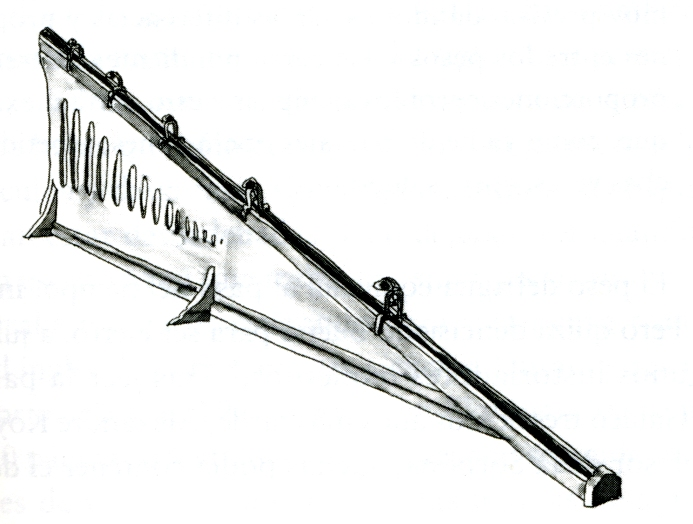
\includegraphics[scale=0.25]{./pictures/planoInclinado.png}
	Fonte: Galileu, Duas novas ciências, pp. 140-141, trad. Mariconda. P. R. Mariconda \& J. Vasconcelos, Galileu e a nova física, p. 44.
\end{figure}

A demonstraçao de tal experiemento, o qual já foi amplamente validado e estudado ao longo da historia, ainda é de extrema importância principalmente no contexto educacional, pois nos permite observar e compreender os principios fundamentais da fisica clássica além do papél, mas apartir de uma abordagem pratica experimental, auxiliando na fixação do conhecimento e na contrução do raciocinio anlitico e científico.

O objetivo deste relatório é descrever a metodologia utilizada para realizar o experimento de Galileu com um plano inclinado, apresentar os resultados obtidos e discutir as conclusões que podem ser tiradas a partir desses resultados. Através deste experimento, buscamos não apenas determinar o valor da aceleração da gravidade, mas também compreender melhor os princípios do movimento uniformemente acelerado e a influência da inclinação do plano nesse movimento.

% \begin{table}
% 	\centering
% 	\caption{Este é um exemplo de formatação de tabela~\cite{michael}.}
% 	\scalefont{0.9}
% 	\begin{tabular}{|c|c|c|}
% 		\hline
% 		Kelvin (K) & Celsius (ºC) & Fahrenheit (ºF) \\ \hline
% 		271        & 2            & 31              \\ \hline
% 		274        & 5            & 36              \\ \hline
% 		277        & 8            & 39              \\ \hline
% 		281        & 11           & 42              \\ \hline
% 	\end{tabular}\\
% 	\label{table1}
% \end{table}

% Lembre-se de colocar a figura e a tabela~\ref{table1} centralizadas na coluna assim como seus textos descritivos (legendas). Esses textos descritivos devem ser sucintos, objetivos e claros de forma que a pessoa que vê a figura ou tabela saiba do que se trata.

\section{Metodologia}
Nesta seção são descritos os procedimentos empregados para efetuar as medidas e são descritas as montagens experimentais utilizadas. Diagramas esquemáticos das experiências são bastante úteis pois facilitam a visualização.  Este procedimento NÃO é uma cópia do roteiro do experimento pois o mesmo não contém detalhes relevantes que somente podem ser percebidos durante a elaboração da experiência. Lembre-se que seu leitor deve ser capaz de reproduzir o experimento a partir da leitura desta seção e da seção~\ref{intro}.

\section{Resultados e Discussões}
Esta seção é o coração do relatório. Nela são apresentados os dados obtidos em forma de tabelas, gráficos e diagramas. Lembre-se que quando o volume de dados é elevado os gráficos devem ter preferência sobre as tabelas. Os resultados experimentais devem ser confrontados com as previsões teóricas e com os resultados existentes na literatura citada na introdução. Quando são efetuados cálculos complexos não é necessário descrever todas as etapas do processo. No caso dos resultados experimentais, dentro das estimativas de erro, apresentarem discrepâncias com as previsões teóricas o procedimento experimental deverá ser reavaliado (isto porque no nosso caso os resultados são muito bem conhecidos). Na vida real pode ocorrer discrepância devido às falhas dos modelos teóricos existentes, ou das medidas feitas previamente. Lembre-se que toda medida experimental apresenta incerteza e portanto as contas efetuadas devem levar estas em consideração.

\begin{figure}[!htpb]
	\centering
	\caption{Velocidade em função do tempo.}
	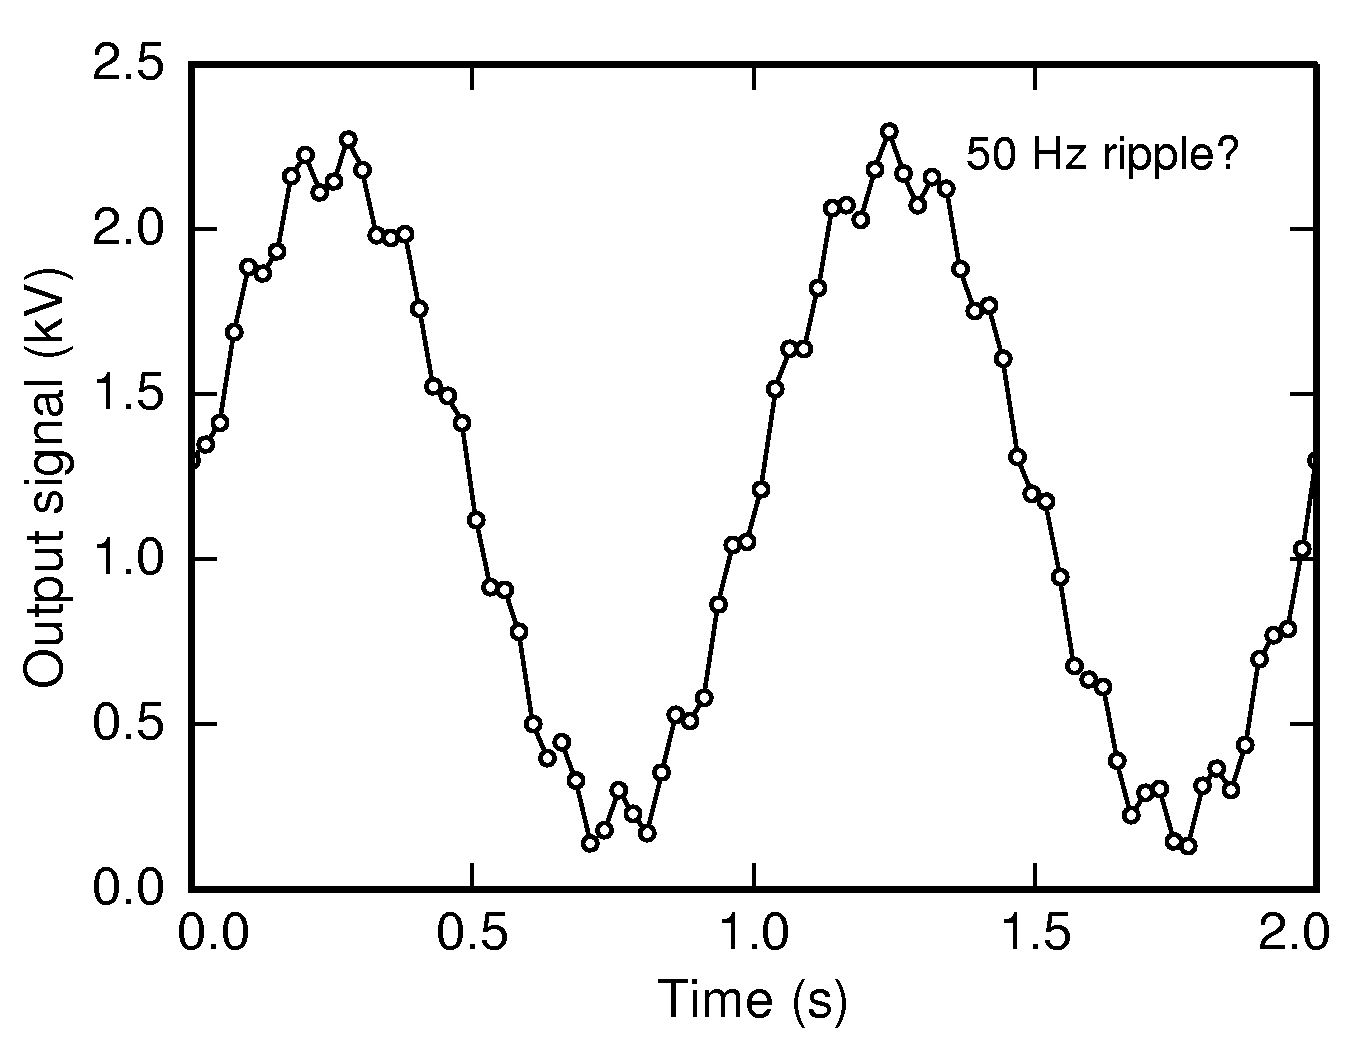
\includegraphics[scale=0.15]{./pictures/grafico1.png}
	Fonte: Adaptado do Halliday e Resnick~\cite{Halliday-II}.
\end{figure}

\section{Conclusão}
A conclusão deve abordar brevemente o experimento efetuado, os resultados obtidos e a que conclusões estes resultados levam. Em alguns casos se discute possíveis rumos desta investigação. Comentários do tipo: ``O experimento foi muito proveitoso$\dots$'' e outro similares deve ser evitados.

%\onecolumn

\bibliographystyle{unsrt}
\bibliography{biblio.bib}

\end{document}